
%
%  $Description: Author guidelines and sample document in LaTeX 2.09$ 
%
%  $Author: ienne $
%  $Date: 1995/09/15 15:20:59 $
%  $Revision: 1.4 $
%

\documentclass[times, 10pt,twocolumn]{article} 
\usepackage{epsfig}
\usepackage{latex8}
\usepackage{times}
\usepackage{url}

%\documentstyle[times,art10,twocolumn,latex8]{article}

%------------------------------------------------------------------------- 
% take the % away on next line to produce the final camera-ready version 
\pagestyle{empty}

%------------------------------------------------------------------------- 
\begin{document}

\title{User-level Grid Monitoring with Inca 2}

\author{Shava Smallen, Kate Ericson, Jim Hayes, Catherine Olschanowsky \\
San Diego Supercomputer Center\\ University of California, San Diego\\ 
9500 Gilman Drive, La Jolla, CA 92093-0505, USA\\ 
\{ssmallen,kericson,jhayes,cmills\}@sdsc.edu\\
}

\maketitle
\thispagestyle{empty}

%1.  Motivate and differentiate the Grid monitoring Inca does
%2. Describe Inca 2 design and its benefits
%3. Illustrate that Inca 2 design is mature and being used in production by
%several Grids
%4. Be different from Inca 1 paper

\begin{abstract}
User-level Grid monitoring is valuable, how it relates to other Grid
monitoring,  and what are its implementation challenges.
Inca 1 good but had limitations.  In this paper, we introduce Inca 2 and
describe its features and architecture.  We then show a few use cases for Inca
is being deployed on TeraGrid and XXX?  System impact results and performance
results.  Finally, we discuss our future work.  
\end{abstract}

%------------------------------------------------------------------------- 
\Section{Introduction}

% Standard "Grids are good" intro paragraph.  But are complex.  
Grid systems provide unified and coherent access to distributed computing,
data storage and analysis, instruments, and other resources.  These systems
require the careful coordination of software packages, services, and
configurations across multiple, heterogenous resources.  The TeraGrid
project~\cite{teragrid}, for example, manages the coordination of software and
services by deploying and monitoring a common user environment across
distributed, heterogeneous resources. The organization of TeraGrid software
and services is referred to as the Common TeraGrid Software and Services
(CTSS).  TeraGrid's software and services uniformity simplifies access to its
resources, which consist of more than 102 teraflops of compute capability and
more than 15 petabytes of online storage, all interconnected by a network that
can transfer a terabyte of data in under 10 minutes.  

% Complex means they are difficult to provide and maintain. Describe the
% stakeholders.   Monitoring is needed.
Providing and maintaining a stable infrastructure for these complex 
Grid systems poses challenges for both administrators who build and
maintain Grid resources and scientists who use them.  
% Why?  
% 1. Administration is distributed across multiple admins
Administration of the Grid infrastructure is typically coordinated by a group 
of Grid operators who decide when software should be deployed to resources and
how it should be configured.  Each site's system administrators are then
responsible for providing the required software components and services for
their resource.  Grid operators need to take into account local site policies
and heterogenous architectures when requiring software.  System administrators
need to learn enough Grid knowledge to deploy software and debug problems.  In
this distributed model, good communication of the requirements is required in
order for Grid resources to interoperate with one another.  Otherwise
inconsistencies between the resources arise that can either inconvenience the
user or prevent them from using particular resources together.
% 2. Grid software failures
distributed system, components will fail over time.  As with any distributed
systems, the probability of failure increases as the number of elements 
increase.  Failures can occur due to system downtimes, misconfiguration in the 
software, bugs in the software, high load.  
which means miscommunications can occur.  
% 3. Changes 
Third it is challenging due to the
activeness in Grids, packages and updates can occur frequently.

% What types of Grid monitoring are around?  What user-level monitoring
% provides and why we think it is good
One approach to monitoring Grids, used by tools such as
MonALISA~\cite{monalisa} and GridICE~\cite{gridice}, is to aggregate and
display data from existing cluster or system administrator monitoring tools
such as Ganglia~\cite{ganglia}, CluMon~\cite{clumon}, and
Nagios~\cite{nagios}.  This provides a centralized, systems-level view of Grid
resources where low-level host statistics and queue information can be
examined.  This type of monitoring information is useful for showing the
utilization of Grid resources, however, it does not provide the type of
high-level monitoring needed to detect user problems within the Grid
infrastructure, such as incompatible software versions.  User-level
Grid monitoring approaches testing is important because it run commands that users use and tests
to see if they operate as expected. Execute commands published in user
documentation, detect problems otherwise reported by users.

so called user-level Grid monitoring is bIn our view, what was
needed was a separate
monitoring system to perform automated, periodic user-level Grid testing with
the following features:
User-level Grid monitoring is x and is valuable.  
At that
time, the only available user-level Grid monitoring tools were the NCSA
TestGrid script [9] and GITS [10], scripts that run a fixed number of Grid
tests and output results in HTML.  Although these tools were easy to install
and produced useful information, they showed only the view of the Grid from a
single resource, lacked automation, and were not easily extensible.  

% Inca 1~\cite{inca1} first addressed user-level Grid monitoring but had
% limitations.  We learned lessons from our TeraGrid deployment.  
In 2003, SDSC, in partnership with TeraGrid, began developing the Inca
monitoring tool to implement a user-level monitoring system with the above
features and started using it to validate and verify that CTSS was deployed
consistently across all TeraGrid resources and to monitor its status.  
The initial version of Inca was implemented as a client-server architecture.
It provided data collection, data storage (with limited archiving
capabilities) that was accessible from a Web services interface, and data
display though Web status pages.  Inca was first deployed to TeraGrid in mid
2003 and released in late 2003. After running Inca 1 for a year and a half on
TeraGrid, we learned some valuable lessons and designed Inca version 2, our
current release.  Inca 2 contains a number of substantial improvements over
Inca 1 with respect to security, installation and maintenance, and storage
capabilities.  A pre-release of Inca 2 was provided in February 2006 and a
beta release in November 2006.  A production version of Inca 2 was released in
January 2007.  Currently, seven other Grids in the U.S., Europe, and Australia
use Inca.  

% This motivated our development of a new version of Inca.
In the next section, we describe our experiences with deploying Inca 1 to
TeraGrid and the lessons learned.  We then describe the Inca 2 architecture
and the benefits it provides.  Use cases illustrate that Inca 2 is being used
today and has great results.

\Section{Features}
  
% Philosophy of user-level testing
% Practical byproducts

1.  Periodic tests executed by the monitoring system should be automated and
run from a standard user account.  A user GSI credential should be issued and
used by the monitoring system to test services that require authentication.  
%myproxy stuff
2.  Tests should be executed locally on all Grid resources when appropriate so
that all Grid access points available to users are tested.  
3.  The configuration of tests should be managed centrally in order to ensure
consistent testing of the resources, rather than by system administrators who
may not use the same information that is available to users.
4.  The testing system should easily adapt to new resources and testing
requirements.  In our experience, testing has an iterative refinement process
because Grids are dynamic and the software environment changes over time as
packages are upgraded.  Furthermore, it is often difficult to write and deploy
a test perfectly the first time because of portability issues and incomplete
user documentation.   
5.  System administrators should not need to know the details of the
monitoring system in order to troubleshoot problems.  When a problem is
detected the monitoring system should provide system administrators with
sufficient information to locate the problem easily and test repairs.
6.  A history of test results (especially any error messages) should be
retained in order to understand the behavior of their Grid over time. This
history should be available through a flexible querying interface.
7.  A running monitoring system should have a limited impact on the resources
it measures and should be secure.

~\newpage

%------------------------------------------------------------------------- 
%------------------------------------------------------------------------- 
\Section{Architecture}

\SubSection{Overview}
% may not need to leave in here -- intro is assumed to be overview
% Overview of all architecture components -- arch picture
% move text to here I think
1) The user creates a suite using incat and submits it to the agent

2) The agent 
    a) fetches reporters from the reporter repository
    b) creates a reporter manager on each resource
    c) sends the suite and reporters to each reporter manager.

3) Each reporter manager executes reporters according to its schedule and
sends results (reports) to the depot

4) Data consumers display collected data (reports) by querying the depot

\begin{figure*}[Htb]
  \centering
  \mbox{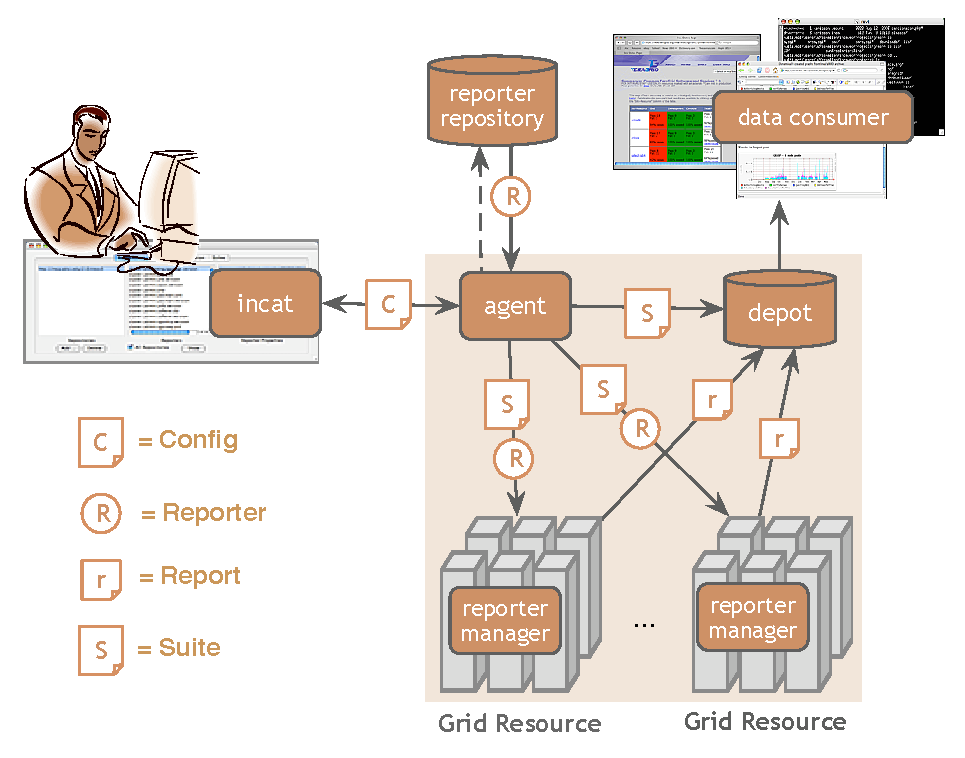
\epsfig{file=arch.eps, width=.8\textwidth}}
  \caption{\label{arch_fig} Inca architecture.}
\end{figure*}

\SubSection{Inca administration GUI tool (incat)}

To configure reporter execution, an Inca administrator launches a GUI tool,
called incat.  Incat allows the administrator to choose which resources to
monitor and which reporters to deploy to those resources.  For each
reporter, the administrator can specify the resources to run on,
command-line arguments, the runtime environment, the frequency of execution,
and resource limits. The Inca administrator may also group related reporters
into suites that can be shared across different Inca deployments.  This can
be useful to determine interoperability among Grids or to determine whether
an application's requirements are being fulfilled on a Grid.

\subsubsection{Reporters}

Each Inca reporter is an executable program that tests or measures some
aspect of a system or installed software.   Reporter executables are
designed to be easy to produce and can be run outside of the Inca system
(e.g., by a system administrator).  A reporter could be a simple Globus
gatekeeper ping test (see Figure 2) or a more complex Grid application
benchmark.  Reporters must support certain command line options and produce
XML according to the Inca reporter schema.  The reporter schema requires a
header describing the context of the reporter execution (e.g., reporter
name, arguments, working directory, timestamp) and a body containing the
results expressed as any XML sequence. This flexible body schema enables
reporters to express a wide variety of information.  Today, we have three
standard body schemas to express software version information, software
functionality or service tests results, and usage information.  We provide
Perl APIs to handle much of the effort of writing reporters.  Most current
reporters use these APIs and consist of fewer than 30 lines of code.  
% capture context of execution

\subsubsection{Reporter Repositories}

The Inca agent retrieves reporters from collections called reporter
repositories, that consist of reporters, required packages and libraries,
and a catalog file. Repository contents are accessible using a URL and can
be shared across multiple Inca deployments. The Inca team publishes a
reporter repository that contains reporters developed for TeraGrid.  

\subsubsection{Suites}
%\subsubsection{Series}

\subsubsection{Resource Macros}

\SubSection{Agent}

The Inca agent is a server that implements the configuration specified by the
Inca administrator.  After determining which Inca tests should be executed on
each resource, the agent stores this configuration information in the depot.
It then stages and launches a dependent component, called a reporter manager,
on each resource using either SSH or Globus [13].  Once a reporter manager
contacts its agent, the agent transmits Inca tests to execute, along with
their dependencies, configuration and schedule of execution. 
  

\SubSection{Reporter Manager}

The Inca reporter manager is a lightweight process responsible for managing
the schedule and execution of Inca tests, called reporters, on a single
resource. The reporter manager receives reporter updates and dependencies
(e.g., Inca Perl APIs or source code) from the agent along with requests for
reporter scheduling changes.  Running under a regular user account, the
reporter manager executes reporters on-demand or using an internal cron
scheduler, and sends reports to the depot for archiving. The reporter
manager monitors reporter system usage and enforces limits (e.g., wall clock
time, CPU time, memory).  System usage information is sent to the depot with
each report. 



\SubSection{Depot}

The Inca depot server is responsible for storing configuration information
and the data produced by reporters. The depot maintains a relational
database via Hibernate [14] so that it can use a variety of databases.  The
depot provides full archiving of reporter output and structures its schema
to reduce redundant data.  Data can be queried using SQL queries. Predefined
queries exist to return the latest report instances of a suite, a single
report instance, or a report history.  A Web services interface is also
available to provide unauthenticated query access to data.  


\SubSection{Data Consumer}

The Inca data consumer is a Web application that queries the Inca depot for
data and displays it in a user-friendly format.  The data consumer is
packaged with Jetty [15] so that pages can be served immediately without
deploying Tomcat [16].  A set of JSP tags and pages query the Inca depot for
data (returned as XML) and a set of XSL stylesheets format the data as HTML.

~\newpage
~\newpage
~\newpage
~\newpage
%------------------------------------------------------------------------- 

\Section{Use Cases}

\SubSection{TeraGrid}

\subsubsection{Description and Requirements}

% Describe CTSS 

\subsubsection{Usage of Inca}

% Describe reporters, configuration, and deployment.  Figure.

\subsubsection{Results}

% Consumer view of CTSS, security, etc.

~\newpage

\SubSection{GrASP}

\subsubsection{Description and Requirements}

% Describe GrASP probes

\subsubsection{Usage of Inca}

% Used to deploy GrASP probes to Grids.  Probes wrapped as reporters (maybe
% right in future as though we already included GrASP as a dependency cause
% it should be done by June.

\subsubsection{Results}

% A paper.  Interesting that error messages were important.  Predictions?

~\newpage

\SubSection{Other uses}
~\newpage
%------------------------------------------------------------------------- 
\Section{Future Work}

\SubSection{Graphing and Summary Statistics}

\SubSection{Knowledge Base}

\SubSection{Fault Tolerance}
~\newpage

%------------------------------------------------------------------------- 
\Section{Summary}

~\newpage

%------------------------------------------------------------------------- 
\bibliographystyle{latex8}
\bibliography{paper}

\end{document}

